\chapter{深度学习平台——TensorFlow}
\chaptermark{深度学习平台——TensorFlow}
	\section{TensorFlow简介}
	2015年11月Google在Github开放TensorFlow的源代码,从此,它已经成为GitHub上最受欢迎的机器学习库。TensorFlow是第二代分布式机器学习算法实现框架及部署系统,是基于使用DisBelief时的经验及训练大规模分布是神经网络的需求开发的。但是在某部分基准上,TensorFlow的性能是DistBelief的两倍。可以方便地部署到各种平台,大大简化了真实场景中应用机器学习的难度。TensorFlow的计算可以表示为有状态的数据流式图,使用数据流式图来规划计算流程,可以将计算映射到不同的硬件和操作系统平台。对于大规模的神经网络训练,TensorFlow可以让用户简单地实现并行计算,同时使用不同的硬件资源进行训练,同步或异步地更新全局共享的模型参数和状态。
	TensorFlow是相对高阶的机器学习库,用户可以方便的用它设计神经网络结构,支持自动求导,核心代码是用C++编写的,简化了线上部署的复杂度,可以在手机和CPU这种内存紧张的设备上运行。除了C++接口外还有Java、Python、Go等接口。TensorFlow可以部署在一台或多台CPU、GPU的机器上,兼容多种平台,包括Android、Windows、Linux等。有TF.Learn和TF.Slim等上层组件可以帮助快速的设计新网络,并且兼容Scikit-learn estimator接口,同时TensorFlow不仅仅局限于神经网络和数据流式图并支持非常自由的算法表达,只要可以将计算表达成计算图的形式,就可以使用TensorFlow。
	另一个重要特点是可以灵活的移植性,可以将同一份代码几乎不经过修改就轻松的部署到任意数量CPU或GPU的PC上、服务器或者移动设备上。还有一个优势就是编译速度极快,在创建新的网络结构时,Theano通常需要很长时间的进行编译,因此尝试新模型需要付出较大的代价,而TensorFlow不存在这样的问题。而且还有功能强大的TensorBoard,能够将网络结构和训练过程进行可视化,对于研究者记录和观察复杂的网络结构和监控长时间、大规模的训练有很大的帮助。TensorFlow不仅支持常见的神经网络结构外,而且还支持深度强化学习甚至支持密集的科学计算。TensorFlow之前版本不支持symbolic loop,需要使用Python循环解决这些问题,从而带来无法进行图编译优化等一系列问题,但最近新发展的XLA开始对JIT及AOT进行支持,另外其使用bucketing trick也可以较高效地实现循环神经网络。TensorFlow的一个不占优势的方面,可能对于计算图必须构建为静态图,这使得很多计算实现困难。
	\begin{figure}[!ht]
		\centering
		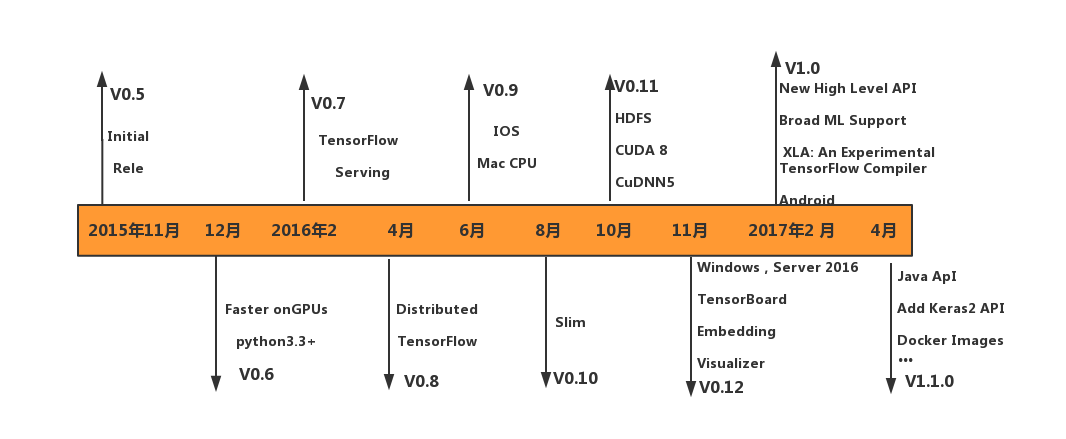
\includegraphics[width=0.5\textwidth]{figures/2-1}
		\caption{TensorFlow发展史}
	\end{figure}
	\section{核心概念}
		\subsection{计算图}
		计算图是TensorFlow中最基本的概念之一,在TensorFlow中的所有计算都会被转化为计算图上的节点。在TensorFlow中计算可以表示为一个有向图(directed graph)或者称为计算图(computation graph)。 
		TensorFlow是一个通过计算图的形式来表述计算的编程系统,其中每一个运算操作(operation)将作为一个节点(node),节点与节点之间的连接成为边(edge)。计算图中每一个节点可以有任意多个输入和任意多个输出,节点可以算是运算操作的实列化。在计算图的边中流动(flow)的数据被称为张量(Tensor),这个也是Tensoflow名字的由来。没有数据流动的边被称为依赖控制。计算图描述了张量数据的计算流程,负责维护和更新状态,对分支进行条件控制和循环操作。如果机器上有超过一个可用的 GPU, 除第一个外的其它 GPU 默认是不参与计算的. 为了让 TensorFlow 使用这些 GPU, 你必须将 op 明确指派给它们执行. with...Device 语句用来指派特定的 CPU 或 GPU 执行操作
		\begin{figure}[!ht]
			\centering
			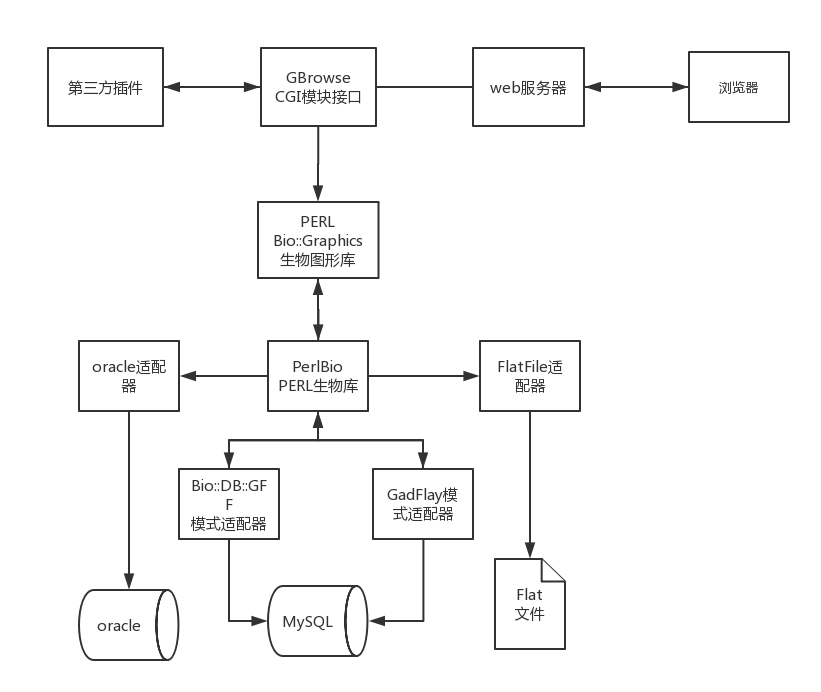
\includegraphics[width=0.5\textwidth]{figures/2-2}
			\caption{计算图示例}
		\end{figure}
		
		\subsection{运行模型}
		Tensorflow的运行环境使用的是Session。用户通过使用TensorFlow交互式接口Session进行操作。
		TensorFlow程序运行时的所有资源由Session管理。当所有计算完成之后需要关闭会话来帮助系统回收资源,否则就可能出现资源泄漏的问题。TensorFlow中使用Session的模式一般有两种,第一种模式需要明确调用会话生成函数和关闭会话函数,第二种模式是通过Python的上下文管理器来使用会话,这种模式为了解决异常退出时资源释放的问题,TensorFlow的会话不会自动生成默认的会话,需要手动指定,当默认的会话被指定之后可以通过tf.Tensor.eval()函数计算一个张量的取值,在交互式环境下(比如Python脚本等)通过设置默认会话的方式来获取张量的取值更加方便,函数tf.InteractiveSession()在交互式环境下直接构建默认会话。使用这个函数会自动将生成的会话注册为默认会话。可以省去将产生的会话注册为默认会话的过程,不论采用哪种方法都可以通过ConfigProto Protocol Buffer来配置生成需要生成的会话,通过ConfigProto可以配置类似并行的线程数,GPU分配策略,运算超时时间等参数。在这些参数中最常使用的是allow\_soft\_placement=和log\_device\_placement两个参数其都是布尔型的参数。 
		在实现上, TensorFlow将图形的定义转换为分布式执行的操作,是为了充分使用可用的计算资源(如 CPU 或 GPU)。 通常来说不需要显式指定使用 CPU 还是 GPU, TensorFlow 能主动检测。如果检测到 GPU, TensorFlow会使用找到的第一个GPU来执行操作。
		
		\subsection{数据模型}
		张量是TensorFlow管理数据的形式,可以被简单的理解为多维数组。其中零阶张量表示标量(scalar),也就是一个数;第一阶张量为向量(vector),也就是一个一维数组;第n阶张量可以理解为一个n维数组。在张量中并没有真正存储数字,它存储的是如何计算得出这些数字的过程。TensorFlow计算结果不是一个具体的数字,而是一个张量的结构,一个张量主要有三个属性:名字(name),维度(shape),类型(type) 
		第一个属性名字不仅仅是张量的唯一标识符,还给出了这个张量是如何计算出来的,张量与计算图上节点代表的计算结果是相对应的,张量的命名能够由“node:src\_output”的方式给出,其中节点的名称为node,src\_output表示当前张量是来自节点的第几个输出。 
		第二个属性是张量的维度(shape)描述了一个张量的维度信息。 
		第三个属性是类型(type)每一个张量会有一个唯一的类型,TensorFlow会对参与运算的所有张量进行类型检查,当发现类型不匹配时会报错。 
		TensorFlow支持多种不同的类型,主要包括了实数(tf.float16 tf.float32,tf.float64)、整数(tf.int16,tf.int32,tf.int64,tf.int8,tf.uint16,tf.uint8)、布尔型(tf.bool),复数型(tf.complex64,tf.complex128)等。 对于张量的使用,可以分为两大类。第一类是对中间计算结果的引用。当一个九三包含很多中间结果时,使用张量可以大大提高代码的可读性。第二类是当计算图构造完成之后,张量可以用来获得计算结果,结合会话使用tf.Session().run(result)就可以得到真实的数字.
		\subsection{变量}
		在TensorFlow中,变量的作用就是保存和更新神经网络的参数。变量包含张量 (Tensor)存放于内存的缓存区。建模时它们需要被明确地初始化,模型训练后它们必须被存储到磁盘。这些变量的值可在之后模型训练和分析是被加载。 TensorFlow提供了一个通过变量名来创建或者获取一个变量的机制。通过这个机制,在不同的函数中可以直接通过变量的名字来使用变量,而不需要将变量通过参数的形式到处传递,这个机制主要通过tf.get\_variable()和tf.variable\_scope()函数实现的。
	\section{Tensorflow环境搭建}
	Tensorflow对各种主流的操作系统的支持都比较完善,本文将使用Tensorflow对Python提供的API进行研究学习。Tensorflow支持的Python环境有Python2.7和Python3.5,目前最新版本的Tensorflow支持Python3.5。Tensorflow环境的搭建可以分为两类,第一种是使用官方提供的发行进行安装使用,第二种是下载Tensorflow的源代码进行编译安装使用。本文将以第一种方式在Linux和Windows系统环境下分别使用Pip和Anaconda进行环境搭建。
		\subsection{Pip下环境搭建}
		Pip是一个以Python计算机程序语言写成的软件包管理系统,其可以安装和管理软件包。通过Pip可以安装已经打包好的TensorFlow以及TensorFlow所依赖的其他Python扩展包。环境需保证操作系统上有Python的环境,首先,安装Python的Pip包,然后通过Pip命令针对不同版本的Python安装CPU或者GPU版本的Tensorflow。如下安装过程的详细代码。
		\begin{lstlisting}
		 sudo apt-get install python-pip python-dev
		 pip install tensorflow  # Python 2.7; CPU support (no GPU support)
		 pip3 install tensorflow # Python 3.n; CPU support (no GPU support)
		 pip install tensorflow-gpu  # Python 2.7;  GPU support
		 pip3 install tensorflow-gpu # Python 3.n; GPU support
		\end{lstlisting}
		\subsection{Anaconda下环境搭建}
		Anaconda是由Python开发的领先的开放数据科学平台。 包括超过100种最受欢迎的数据科学Python,R和Scala软件包。内置了大量的Python经常用的库,包括SciPy、Numpy、Scikit-learn、Pandas等。 首先,需要安装用于科学计算的Anaconda环境,其次创建Python不同版本的环境,最后通过使用Python的包管理工具Pip安装TensorFlow的环境。安装过程的详细代码如下。图2-2安装成功后测试图。
		\begin{lstlisting}
		Anaconda3-4.3.1-Windows-x86_64.exe #Windows Install
		bash Anaconda3-4.3.1-Linux-x86_64.sh #Linux Install
		conda create --name python35 python=3.5 # create environment in Linux and Windows
		source activate Python35 # Linux
		activate Python35 #Windows
		pip install tensorflow #install TensorFlow
		\end{lstlisting}
		
		\begin{figure}[!ht]
			\centering
			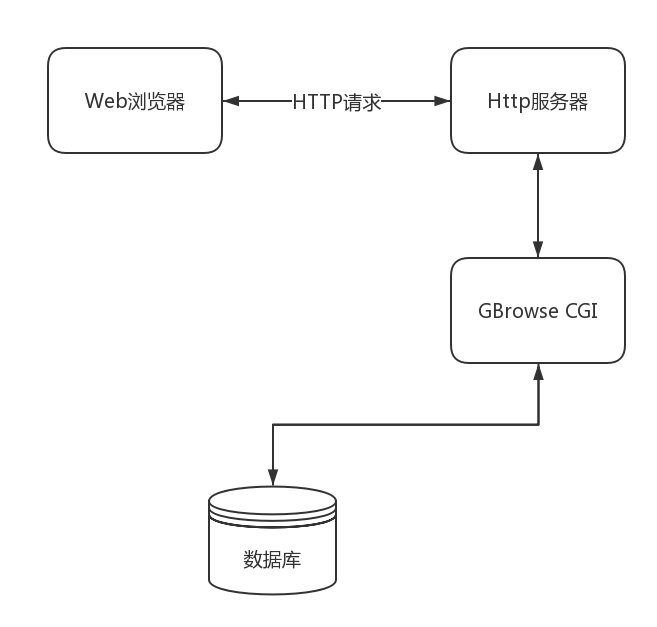
\includegraphics[width=0.8\textwidth]{figures/2-3}
			\caption{TensorFlow安装成功}
			\label{fig:2-3}
		\end{figure}